\part*{Desarrollo}

% ====================================================== %

\section{Definición del proyecto}

\lipsum[10]

% ====================================================== %

\section{Modelado del Sistema}

% ====================================================== %

\subsection{Traslación del Carro}

Como ya se menciono subsistema de traslación del carro es el encargado de 
mover la carga sobre el puente de la grúa portuaria desde el barco hasta 
el muelle y viceversa en el proceso de carga y descarga de mercancías.

El carro esta simplemente apoyado sobre sus 4 ruedas, no motorizadas, en 
los rieles de la viga principal del puente de la grúa portuaria, 
por lo que se considera que solo puede desplazarse horizontalmente y 
sin resbalamiento.

Su desplazamiento se da por los cables ubicados en sus laterales. Estos
cables trabajan en paralelo y se despliegan en una configuración cerrada
desde el carro hasta el tabor que se encentra en la casa la 
casa de maquinas. El tambor es el elemento que transforma el movimiento
oracional de los motores en movimiento lineal del carro.

Dentro de la casa de maquinas también se encentra el motor que acciona el
carro que esta acoplado con un reductor que a vez esta acoplado con el tambor.
En el eje del motor hay un freno de estacionamiento normalmente cerrado, esto
quiere decir que el freno esta activo cuando no tiene energía y se abre
cuando se energiza.

\subsubsection{Carro}

Se puede considerar al carro como un cuerpo rígido que esta simplemente
apoyado sobre una viga y que tiene la capacidad de desplazare libremente
por esta de forma que desde la perspectiva del marco de referencia se
considere solo un movimiento horizontal. Entonces
el diagrama de fuerzas que actúan sobre el carro es el siguiente:

\begin{figure}[H]
    \centering
    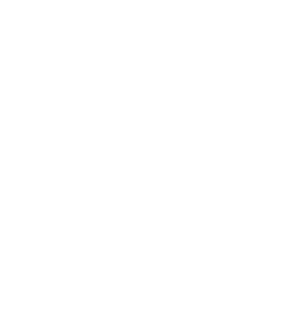
\includegraphics[width=0.5\textwidth]{img/NADA.png}
    \caption{Diagrama de fuerzas del carro}
\end{figure}

La ecuación de movimiento del carro se puede obtener a partir de la segunda
ley de Newton. La ecuación de movimiento es la siguiente:

\begin{equation}
    M_t \ddot{x_t}(t)  = F_{tw}(t) - b_{t} . \dot{x_t}(t) + 2.F_{hw}.sen(\theta(t))
\end{equation}

\subsubsection{Cable del Carro Elástico Amortiguado}

\subsubsection{Accionamiento de Traslación del Carro}

% ====================================================== %

\subsection{Izaje de la Carga}

\subsection{Análisis de la Carga}